\documentclass[10pt]{article}
\usepackage{amsmath,textcomp,amssymb,geometry,graphicx,enumerate,tikz,algorithm,algpseudocode,pifont}
\usetikzlibrary{calc}
\usetikzlibrary{datavisualization}
\usetikzlibrary{datavisualization.formats.functions}


\textheight=9in
\textwidth=7in
\topmargin=-.75in
\oddsidemargin=-0.25in
\evensidemargin=-0.25in

\usepackage{listings}
\lstnewenvironment{codeblock}
    {\lstset{language=Python,
      showspaces=false,
      showtabs=false,
      breaklines=true,
      mathescape=true,
      showstringspaces=false,
      breakatwhitespace=true,
      commentstyle=\textit,
      keywordstyle=\textbf,
      basicstyle=\ttfamily,
      escapechar=`,
      moredelim={**[is][{\color{RoyalBlue}}]{\^^M\\beginsol}{\^^M\\endsol}},
      moredelim={[is][{\color{RoyalBlue}}]{\^^M\\beginexp}{\^^M\\endexp}},
    }}
    {}

\begin{document}
\section*{02/17/2016}
	\subsection*{Eigenvectors}
	\
		\begin{itemize}
			\item Given a matrix A, if $Av = \lambda v$ for some vector $v \neq 0$, scalar $\lambda$, then $v$ is an \underline{eigenvector} of A and $\lambda$ is the associated \underline{eigenvalue} of A.
			
				\begin{center}
					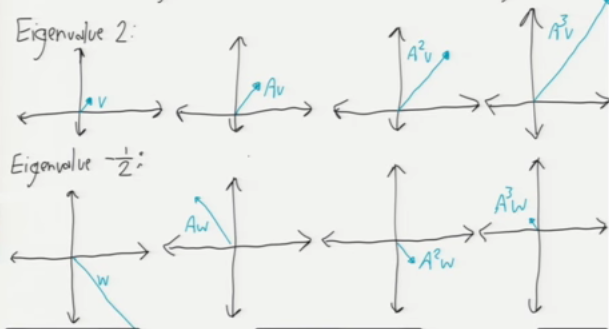
\includegraphics[scale=0.5]{../images/eigenvectors}
				\end{center}
			\item Theorem: if $v$ is an eigenvector of A with eigenvalue $\lambda$, then $v$ is an eigenvector of $A^{k}$ with eigenvalue $\lambda^{k}$.
			\item Proof: $A^{2}v = A(\lambda v) = \lambda^{2}v$ etc.
			\item Theorem: moreover, if $A$ is invertible, then $v$ is an eigenvector of $A^{-1}$ with eigenvalue $\frac{1}{\lambda}$.
			\item Proof: $A^{-1}v = \frac{1}{\lambda}A^{-1}Av = \frac{1}{\lambda}v$.
			\item \underline{Spectral Theorem}: Every symmetric $nxn$ matrix has $n$ eigenvectors that are mutually orthogonal,
				\begin{align*}
					v_{i}^{T}v_{j} = 0, \forall i\neq j
				\end{align*}
			\item We can use them as a basis for $\mathbb{R}^{n}$.
				\begin{center}
					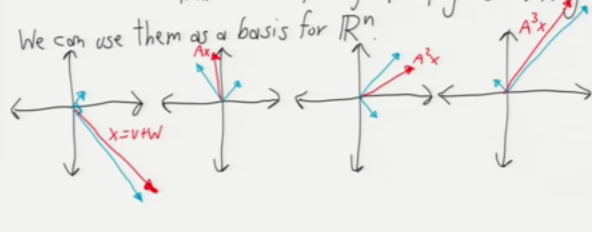
\includegraphics[scale=0.5]{../images/basis}
				\end{center}
			\item Write $x$ as a linear combination of eigenvectors:
				\begin{align*}
					x &= \alpha v + \beta w\\
					A^{k}x &= \alpha \lambda_{v}^{k} v + \beta \lambda_{w}^{k} w\\
				\end{align*}
			\item \underline{Ellipsoids}
				\begin{align*}
					f(x) &= x^{T}x \Leftarrow \text{quadratic; isotropic; isosurfaces are spheres.}\\
					g(x) &= f(Ax) \Leftarrow A \text{symmetric}.\\
					  	&= x^{T}A^{2}x \Leftarrow\text{\underline{quadratic form} of the matrix} \ A^{2} \ \text{anisotropic; isosurfaces are ellipsoids}\\
				\end{align*}
				\begin{center}
					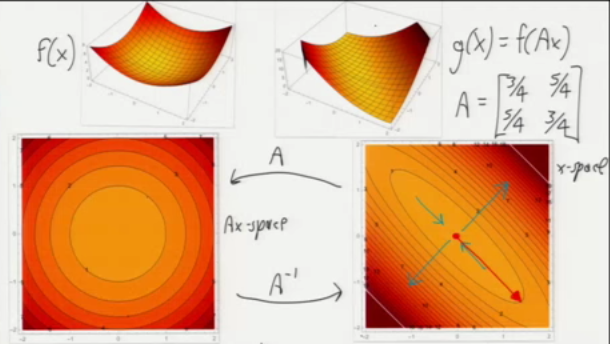
\includegraphics[scale=0.7]{../images/ellipses}
				\end{center}
				\begin{itemize}
					\item $g(x) = 1$ is an ellipsoid with axes $v_{1}, v_{2}, \dots, v_{n}$  and radii $\frac{1}{\lambda_{1}}, \frac{1}{\lambda_{2}}, \dots, \frac{1}{\lambda_{n}}$ (eigevalues of A) because if $v_{i}$ has length $\frac{1}{\lambda_{i}}$ (red arrow), $g(v_{i}) = f(\lambda_{i}v_{i}) = 1 \Rightarrow v_{i}$ lies on the ellipsoid.
				\end{itemize}
			\item Bigger eigenvalue $\Leftrightarrow$ steeper slope $\Leftrightarrow$ shorter ellipsoid radius.
			\item Alternative interpretation:
				\begin{itemize}
					\item Ellipsoids are spheres in a \unexpanded{distance metric} $A^{2}$.
					\item Call $M = A^{2}$ a \underline{metric tensor} because the distance between samples $x$ and $z$ in stretched space is $d(x, z) = |Ax - Az| = \sqrt{(x-z)^{T}M(x-z)}$.
					\item Ellipsoids are "spheres" in this metric: $\{x: d(x, \text{center}) = \text{isovalue}\}$.
				\end{itemize}
			\item A square matrix $B$ is,
				\begin{itemize}
					\item \underline{positive definite} if $w^{T}Bw > 0$ for all $w \neq 0 \Leftrightarrow$ all positive eigenvalues.
					\item \underline{positive semidefinite} if $w^{T}Bw \geq 0$ for all $w \neq 0 \Leftrightarrow$ all non-eigenvalues.
					\item \underline{indefinite} if at least one positive eigenvalue and one negative eigenvalue.
					\item \underline{invertible} if no zero eigenvalue.
					\begin{center}
						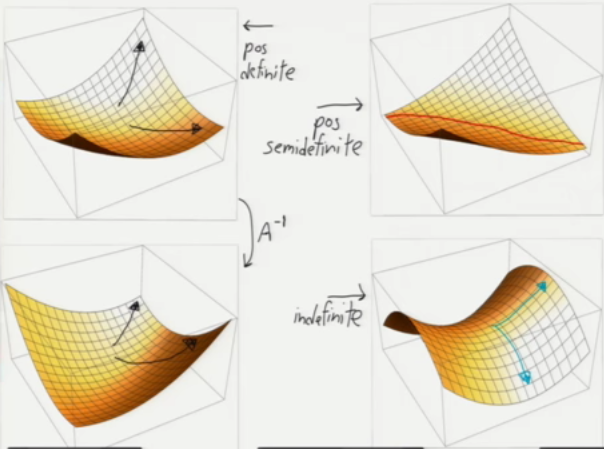
\includegraphics[scale=0.5]{../images/matrices}
					\end{center}
				\end{itemize}
			\item Metric tensor must be symmetric positive definite (SPD).
			\item Special case: $M$ and $A$ are diagonal matrices $\Leftrightarrow$ eigenvectors are coordinate axes $\Leftrightarrow$ ellipsoids are axis-aligned.
		\end{itemize} 
	
	\subsection*{Building a Quadratic with specified eigenvectors and eigenvalues}
		\
		\begin{itemize}
			\item Choose $n$ mutually orthogonal unit n-vectors $v_{1}, \dots, v_{n}$ Let, $V = [v_{1}, v_{2}, \dots, v_{n}]$
			\item Observe: $V^{T}V = I \Rightarrow V^{T} = V^{-1} \Rightarrow VV^{T} = I$.
			\item $V$ is \underline{orthogonal matrix}: acts like rotation (or reflection).
			\item Choose some inverse radii $\lambda_{i}$:
			\item Let,
				\begin{align*}
					\Lambda =
						\begin{bmatrix}
							\lambda_{1} & 0 & \dots & 0\\
							0 & \lambda_{2} & \dots & 0\\
							\vdots & & \ddots & \vdots &\\
							0 & 0 & \dots & \lambda_{n}\\
						\end{bmatrix}
				\end{align*}
			\item Theorem: $A = V\Lambda V^{T} = \sum_{i=1}^{n} \lambda_{i} v_{i}v_{i}^T$ has chosen eigenvectors and eigenvalues.
			\item Proof: $AV = V\Lambda \Leftarrow$ definition of eigenvectors! (in matrix form).
			\item This is a \underline{matrix factorization} called the \underline{eigen-decomposition}
			\item $\Lambda$ is the diagonalized version of $A$.
			\item $V^{T}$ rotates the ellipsoid to be axis-aligned.
			\item This is also a recipe for building quadratics with axes $v_{i}$, radii $\frac{1}{\lambda_{i}}$.
			\item Given SPD metric tensor M, we can find symmetric \underline{square root} $A = M^{\frac{1}{2}}$:
				\begin{itemize}
					\item compute eigenvectors and eigenvalues of $M$
					\item take square roots of $M's$ eigenvalues
					\item reassemble matrix $A$.
				\end{itemize}
		\end{itemize}
\end{document}